\documentclass{article}
\usepackage{hyperref}
\usepackage{fancyvrb}
\usepackage{fvextra}
\usepackage{ragged2e}
\usepackage{enumitem}
\usepackage{pifont}
\usepackage{Tabbing}
\usepackage[utf8]{inputenc}
\usepackage{graphicx}


\title{          \textbf{
                        OS 211        \\*
                    TASK 1: SCHEDULING  \\*
                    DESIGN DOCUMENT }}
\author{Ioana-Cristina Mocanu icm19@ic.ac.uk\\* Vlad Nicolaescu vn119@ic.ac.uk\\*Tudor Udriste tu219@ic.ac.uk\\* Andrei-Oliviu Sologon as5519@ic.ac.uk}

\begin{document}

\maketitle

\section*{PRIORITY SCHEDULING}

\subsection*{DATA STRUCTURES}
\justify

A1:\\*
struct members added in \textbf{struct thread}:
\begin{itemize}
\item \textbf{struct list donations};							/* list of threads that have donated priorities to this thread*/
\\*Represents the list of threads which have donated priority to the current thread
\item \textbf{struct list\_elem donation\_elem};      /* element of list donations */
\\*Represents an element from the list of donations
\item \textbf{struct lock thread\_waits\_lock};				/ threads waits for a lock*/
\\*This variable saves, if any, as a pointer, the lock which the thread waits for (used in nested donation to find out next lock).
\end{itemize}
struct members added in \textbf{struct semaphore\_elem}:
\begin{itemize}
\item \textbf{int sema\_priority};
\\*Using this variable, we save the priority of any given semaphore to make sure that the highest priority thread wakes up first.\\*
\end{itemize}
A2:\\*
  Thread donations are implemented by each thread structure storing a list of
threads which donated their priority to them. When the actual priority of a thread
is queried using \textbf{thread\_get\_priority\_helper()}, the effective priorities of the threads
from which it received donations are computed the same way, recursively. Then, the
maximum value between its received priorities and its own priority is returned.
  In the diagram, priority of t1 is calculated as maximum between L, his own priority,
and the effective priority of t2 which donated to him. The same way priority of t2 is
computed as maximum between M and priority of t3. t3 does not have any donations so the
effective priority it returns is H. Threfore, t2 acquires effective priority H and so does t1.\\*\\*
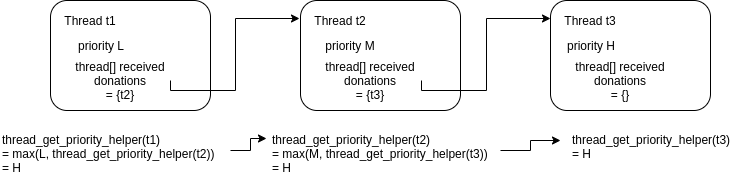
\includegraphics[width=13cm]{nested_donations}

\subsection*{ALGORITHMS}
\justify

A3:
\begin{enumerate}[label=(\roman*)]
  \item Because locks are implemented on top of semaphores (\textbf{sema\_up} is called inside \textbf{lock\_release)},
  the wake up mechanism is inherited from them.\\*
  \item To make sure highest priority waiting thread is selected, in \textbf{sema\_up}, we first
  sort the threads in the list based on their priorities using \textbf{priority\_comp\_func}
  comparator function. Then \textbf{list\_pop\_front()} should return the highest priority
  thread from the waiters list.\\*
  \item Condition variables work in a similar way, but instead of holding a list of sleeping threads,
  they store a list of single-thread semaphores. Therefore, we will store this thread's priority in the
  \textbf{semaphore\_elem} in the list, and when \textbf{cond\_signal()} is called we will first sort the semaphores list
  based on priority of the thread inside them using \textbf{priority\_sema\_comp\_func} comparator function.
  Then, \textbf{list\_pop\_front()} should return the semaphore with the highest priority thread, which will be
  woke up using \textbf{sema\_up()}.
\end{enumerate}
A4:\\*
When calling \textbf{lock\_acquire()} to cause a priority donation, the following sequence of events occurs:
\\*\\*
\textbf{1.} Disable interrupts.
\\*
  \textbf{2.} Donating process.
\\*

     \textbf{2.1}  Checks if lock-\textgreater holder is not \textbf{NULL} (when a donnation occurs, the thread definetely has a holder). If true:
\\*


      \textbf{2.1.1} We set the current thread's waiting lock (\textbf{thread\_waits\_lock}) to this lock.
\\*



      \textbf{2.1.2} We insert in the list of the holder's donations, the donation element of the current thread. We make sure to have the list ordered by priority.
\\*
\\*  \textbf{3.} \textbf{sema\_down} on the lock's binary semaphore controlling access.
\\*
  \textbf{4.} set the current thread to this lock's holder.
\\*
  In this function, for nested donations we only set the lock which is waited by the current thread to the given lock(step 2.1.1).
\\*\\*A5:\\*
When calling \textbf{lock\_release()} on a lock that a higher-priority thread is waiting for, the following sequence of events occurs:\\*
      \textbf{1.} Disable interrupts.
\\*
      \textbf{2.} Checks if the list of waiters is not empty. (and it shouldn't be, followed by the fact that a higher priority thread is waiting for the lock). If true:
\\*

          \textbf{2.1} Removes the donation element of the thread which is ready to wake up. The thread is the first element of the waiters list.
\\*

           \textbf{2.2} Iterates through the list of all donations of the lock's holder.
\\*


            \textbf{2.2.1} If the donated thread waits for the given lock, we remove the thread from the list of donations and add its donation element to the ready-to-wake-up thread's list of donations (nested donation).
\\*
\\* \textbf{3.} We set the lock holder to NULL.
\\*
      \textbf{4.} \textbf{sema\_up} on the lock's semaphore.


\subsection*{SYNCHRONIZATION }
\justify

A6:\\*
We avoid a race condition in \textbf{thread\_set\_priority()} using a lock. The threads are forced to acquire a lock to the thread's \textbf{set\_priority\_lock} before setting the value and release it if and only if the changing of the value is complete. We have to make sure that we do not call this function from interrupt context.

\subsection*{RATIONALE}
\justify

A7:\\*
The design we chose for the priority scheduler is simple and make use of the
most structures that were already used. We store threads in the same waiting lists
as before (\textbf{ready\_list}, \textbf{semaphore-\textgreater waiters} etc.) without unnecessarily extending the
code or using more space. However, for the priority scheduling to work, this lists
have to be maintained sorted at every step.
    We first considerer inserting threads with \textbf{list\_insert\_ordered()} instead of
sorting the list everytime, but there are also cases when a priority is changed
while the thread is inside the list so we have to reassure the list is sorted.
    An alternative to storing all threads in one list ordered by priorities is
grouping the threads by their priorities in 64 priority list. The decision of which
design is better is a matter of what do we want to optimize between time and space,
or time and extensibility, as our implementation uses less space and can be used
to sort threads by any properties, not just 64 priorities.


\section*{ADVANCED SCHEDULER}

\subsection*{DATA STRUCTURES}
\justify

B1:\\*
struct members added in \textbf{struct thread}:
\begin{itemize}
\item \textbf{int nice};
\item \textbf{int recent\_cpu};
\\*We must compute the priority for each thread thus we have to add the "int nice" field in order to hold the niceness and the recent\_cpu field for holding the thread's recent\_cpu value. The priority of each thread is directly dependent on the nice and recent\_cpu value.
\end{itemize}
variables added in \textbf{thread.c}:
\begin{itemize}
\item \textbf{static struct list ready\_list\_mlfqs;};
\\*We created a list to hold the mlfqs ready threads. The threads are ordered by priority. We wanted to split the ready threads as the mlfqs threads should be sorted independently. Otherwise a lower priority thread might be chosen over a higher priority thread.
\end{itemize}
definitions added in \textbf{fixed-point.h}:
\begin{itemize}
\item \#define \textbf{SHIFT} (1 \textless \textless 14)
\item \#define \textbf{ROUND} (SHIFT / 2)\\*

/* Conversion utils: */
\item \#define \textbf{INT\_TO\_FIXED(n)} ((n) * SHIFT)
\item \#define \textbf{FIXED\_TO\_INT(x)} ((x) / SHIFT)
\item \#define \textbf{FIXED\_TO\_INT\_ROUNDED(x)}
((x) \textgreater = 0) ? (((x) + ROUND) / SHIFT) : (((x) - ROUND) / SHIFT)\\*

/* Operations between two fixed-point numbers: */
\item \#define \textbf{ADD\_FIXED\_FIXED(x, y)} ((x) + (y))
\item \#define \textbf{SUB\_FIXED\_FIXED(x, y)} ((x) - (y))
\item \#define \textbf{MUL\_FIXED\_FIXED(x, y)} ((((int64\_t) x) * (y)) / SHIFT)
\item \#define \textbf{DIV\_FIXED\_FIXED(x, y)} (((int64\_t) x) * (SHIFT)) / (y)\\*

/* Operations between fixed-point number and integer: */
\item \#define \textbf{ADD\_FIXED\_INT(x, n)} ((x) + (n) * SHIFT)
\item \#define \textbf{SUB\_FIXED\_INT(x, n)} ((x) - (n) * SHIFT)
\item \#define \textbf{MUL\_FIXED\_INT(x, n)} ((x) * (n))
\item \#define \textbf{DIV\_FIXED\_INT(x, n)} ((x) / (n))\\*\\*
We implemented the fixed points because the floating point arithmetic is not supported by the kernel in pintos. We need the fixed points to calculate the recent\_cpu and load\_avg.
\end{itemize}

\subsection*{ALGORITHMS}
\justify

B2:\\*\\*
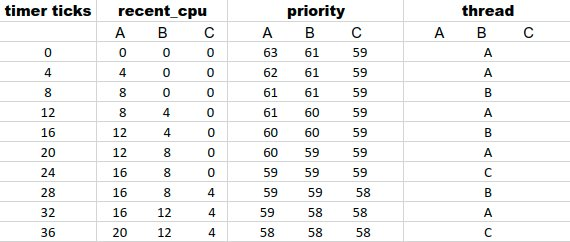
\includegraphics[width=13cm]{img2}
\\*
B3:\\*
One ambiguity found in the specification is the calculation of \textbf{recent\_cpu}. Every 4 ticks, the CPU calculates variables such as recent\_cpu, priorities for all threads in all\_list, load\_avg and sorts the ready\_list.
By doing such, every 4 ticks, the real ticks which are added to recent\_cpu are in fact not 4 ticks due to the fact that the current thread
needs to yield and not run. Not knowing the real value, we add 4 ticks to recent\_cpu every 4 ticks.

Moreover, even though the specification mentions the round robin technique when choosing which thread
to schedule when more threads have the same priority, we believe that it could have been helpful to
have an implementation which also chooses the thread with the smaller recent\_cpu value. We believe that it is more
deterministic and less prone to errors.

\subsection*{RATIONALE}
\justify

B4:\\*
We decided that it is better to create a header for the fixed points instead of an actual C file. The header is more readable this way as all the functions are one liners. Even though the fixed point operations are more precise, they take more time to be computed, so we tried to avoid them where it is not necessary. Hence, if our final result is an integer instead of "x = \textbf{FIXED\_TO\_INT(ADD\_FIX- ED\_INT(y, 100))}" we should write "x = \textbf{FIXED\_TO\_INT(y) + 100}" in order to have a smaller computation time. We made sure that this technique does not influence our results mathematically.

We used another list for the mlfqs ready threads, although considering the fact that the scheduler is either bsd or donation based, any two lists should not be in conflict with each other. One of the lists should be empty at all times. However, in order to make sure that we do not have any bugs due to conflicts rising from list sorting we made a trade off. The disadvantage of this is the fact that we used a bit more memory than necessary, but not considerably more. The advantage of this approach was that we avoided any risk of scheduling a lower priority thread over a high priority thread, a problem that can be caused by a wrongly chosen sorting algorithm.

\end{document}
